\graphicspath{{figures/requirements/}}

\chapter{System Requirements} \label{ch:SystemRequirements}
In this chapter a solution to the problem statement (in \autoref{sec:problem_statement}) is described and a list of requirements for the system is formulated from the findings of the technical analysis. 

\section{Description of solution}
%A ground based system that charges a flying drone wirelessly would be a beneficial solution in today's rising drone market as described in \autoref{sec:app_drones}.
%The designed system is a solution for continuously tracking a flying drone. A laser will be used to verify the precision of the tracking.

%\autoref{fig:use_case} shows a use case diagram of the system.
%\begin{figure} [h!]
%\centering
%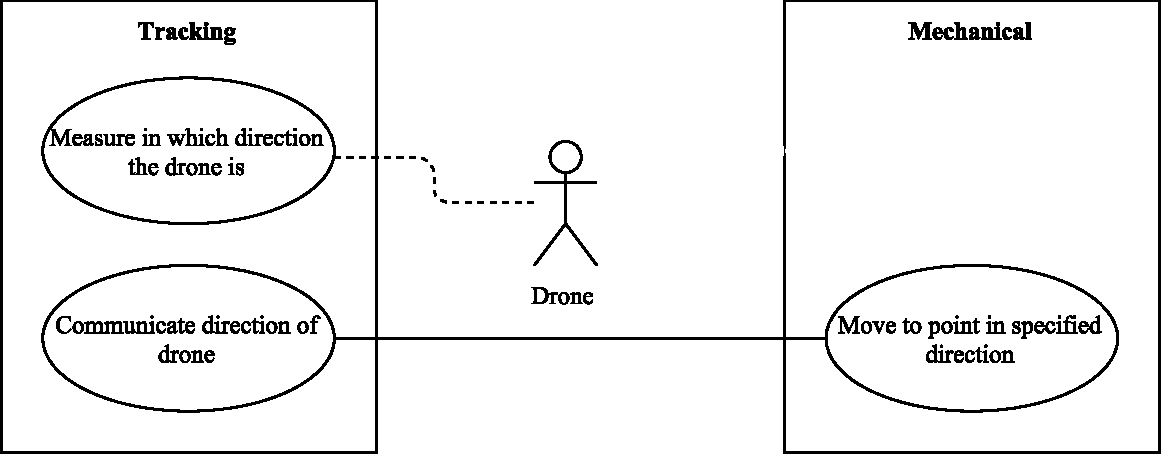
\includegraphics[width=0.7\linewidth]{drone_tracking_use_case_diagram}
%\caption{Use case diagram of the drone tracking platform centred around the drone.}
%\label{fig:use_case}
%\end{figure}

The system consists of a mechanical antenna stand, which have two motors attached to it making it able to rotate and elevate. On the antenna stand a laser pointer and some electrical circuits are to be attached. 

The system is seen at two separate modules, a \textit{tracking module} and a \textit{mechanical module}. 

The tracking module handles the acquiring of the direction of the drone and communicates the direction described in spherical coordinates to the mechanical module. 

The mechanical module moves the antenna stand, making the laser point in the direction specified by the tracking module. The laser should then be pointing directly at the drone in order to simulate the principle of tracking and pointing for use in a wireless power transfer system.

The tracking of the drone happens in real time and the mechanical module should move to the new direction whenever a new direction estimate is received.

Using this description, a set of requirements for the system is made.
%The laser pointer on the stand will rotate and elevate with the stand, this laser pointer will be used to verify the precision of the tracking.

\section{System requirements for the tracking module}\label{sec:systemRequiremetnsTracking}

\reqPrefix{TR}
\reqHeader
\requirement{The tracking module should be able to detect the drone at distances of up to \SI{120}{\meter}.\label{req:track_distance}}{Argued for in \autoref{sec:RequiredPrecision}.}

\requirement{The tracking module should be able to detect the drone at distances of down to \SI{20}{\meter}.\label{req:track_distanceMin}}{Argued for in \autoref{sec:NeedForSpeed}}

\requirement{The tracking module should be able to keep track of a drone moving at speeds up to \SI{24,7}{\meter\per\second}.\label{req:track_speed}}{Based on the speed of drone, found in section \ref{sec:droneSpec}.} 

\requirement{The tracking module must be able to locate the drone with a maximum angular deviation of \SI{2,08}{\milli\radian}.\label{req:track_precision}}{Calculated in \autoref{eq:RequiredPrecision}, \autoref{sec:RequiredPrecision}.}

\requirement{The tracking module should be able to communicate the found angles to the mechanical module\label{req:track_com}}{Design choice to construction and implementation of modules.}

\section{System requirements for the mechanical module}
\bigskip
\reqPrefix{MECH}
\reqHeader

\requirement{The stand should be able to receive pointing instructions from the tracking module \label{req:mech_com}}{Design choice to construction and implementation of modules.}

\requirement{The stand must be able to support a laser\label{req:mech_laser}}{Design choice, for the purpose of testing that tracking module is aimed at the drone.}

\requirement{The stand must point in the indicated direction with a maximum angular deviation of less than \SI{2,08}{\milli\radian} in azimuth angle and less than \SI{2,08}{\milli\radian} in the elevation angle.\label{req:mech_precision}}{Calculated in \autoref{eq:RequiredPrecision}, \autoref{sec:RequiredPrecision}.}

\requirement{The stand should be able to rotate with an angular velocity of up to \SI{1.2361}{\radian\per\second} in the azimuth direction and \SI{1.2361}{\radian\per\second} in the elevation direction.\label{req:mech_speed}}{Calculated in \autoref{eq:NFS4}, \autoref{sec:NeedForSpeed}.}

\section{Compatibility requirements} 
\reqPrefix{COMP}
\reqHeader
\requirement{The entire design should be implemented to fit on the motorised antenna stand.\label{req:mounting}}{Everything should be attached to the available antenna stand described in \autoref{sec:AnalysisMotorisedStand}.}
\requirement{The design should not expose the motors to voltages above their maximum operational values.}{As the motors and mounting solution are tightly coupled, the design should operate within the operating conditions of the motors. Analysis of the motors is done in \autoref{sec:AnalysisMotorisedStand}.}

